\documentclass[10pt,fleqn]{article}
\usepackage{hyperref}
\usepackage{graphicx}


\setlength{\topmargin}{-.75in}
\addtolength{\textheight}{2.00in}
\setlength{\oddsidemargin}{.00in}
\addtolength{\textwidth}{.75in}

\nofiles

\pagestyle{empty}

\setlength{\parindent}{0in}

% new math commands


\setlength{\oddsidemargin}{-0.25in}
\setlength{\evensidemargin}{-0.25in}
\setlength{\textwidth}{6.75in}
\setlength{\headheight}{0.0in}
\setlength{\topmargin}{-0.25in}
\setlength{\textheight}{9.00in}

\makeindex

\usepackage{mathrsfs}

%\usepackage[pdftex]{graphicx}
\usepackage{epstopdf}

\newcounter{beans}

\newcommand{\ds}{\displaystyle}
\newcommand{\limit}[2]{\displaystyle\lim_{#1\to#2}}

\newcommand{\binomial}[2]{\ \left( \begin{array}{c}
                                  #1 \\
                                  #2
                                 \end{array}
                            \right) \
                         }
\newcommand{\ExampleRule}[2]
  {
  \noindent
  \rule{\linewidth}{1pt}
  \begin{example}
    #1
    \label{#2}
  \end{example}
  \rule{\linewidth}{1pt}
  \vskip0.125in
  }

\newcommand{\defbox}[1]
  {
   \ \\
   \noindent
   \setlength\fboxrule{1pt}
   \fbox{
        \begin{minipage}{6.5in}
          #1
        \end{minipage}
        }
   \ \\
  }
\newcommand{\verysmallworkbox}[1]
  {
   \ \\
   \noindent
   \setlength\fboxrule{1pt}
   \fbox{
        \begin{minipage}{6.5in}
           #1
           \ \\
           \vskip0.5in \ \\
           \ \\
        \end{minipage}
        }
   \ \\
  }
\newcommand{\smallworkbox}[1]
  {
   \ \\
   \noindent
   \setlength\fboxrule{1pt}
   \fbox{
        \begin{minipage}{6.5in}
           #1
           \ \\
           \vskip2.5in \ \\
           \ \\
        \end{minipage}
        }
   \ \\
  }
\newcommand{\halfworkbox}[1]
  {
   \ \\
   \noindent
   \setlength\fboxrule{1pt}
   \fbox{
        \begin{minipage}{6.5in}
           #1 \hfill
           \ \\
           \vskip3.25in \ \\
           \ \\
        \end{minipage}
        }
   \ \\
  }
\newcommand{\largeworkbox}[1]
  {
   \ \\
   \noindent
   \setlength\fboxrule{1pt}
   \fbox{
        \begin{minipage}{6.5in}
           #1
           \ \\
           \vskip7.5in \ \\
           \ \\
        \end{minipage}
        }
   \ \\
  }
\newcommand{\flexworkbox}[2]
  {
   \ \\
   \noindent
   \setlength\fboxrule{1pt}
   \fbox{
        \begin{minipage}{6.5in}
           #1
           \ \\

           \vskip#2 \ \\
           \ \\
        \end{minipage}
        }
   \ \\
  }


% symbols for sets of numbers

\newcommand{\natnumb}{$\cal N$}
\newcommand{\whonumb}{$\cal W$}
\newcommand{\intnumb}{$\cal Z$}
\newcommand{\ratnumb}{$\cal Q$}
\newcommand{\irrnumb}{$\cal I$}
\newcommand{\realnumb}{$\cal R$}
\newcommand{\cmplxnumb}{$\cal C$}

% misc. commands

\newcommand{\mma}{{\it Mathematica}}
\newcommand{\sech}{\mbox{ sech}}
 
\newtheorem{theorem}{Theorem}
\newtheorem{example}{Example}
\newtheorem{definition}{Definition}
\newtheorem{problem}{Problem}

\setcounter{secnumdepth}{2}
\setcounter{tocdepth}{4}


\begin{document}
%%%%%%%%%%%%%%%%%%%%%%%%%%%%%%%%%%%%%%%%%%%%%%%%%%%%%%%%%%%%%%%%%%%%%%%%%%%%%%%%
%%%%%%%%%%%%%%%%%%%%%%%%%%%%%%%%%%%%%%%%%%%%%%%%%%%%%%%%%%%%%%%%%%%%%%%%%%%%%%%%
\vskip0.1in\hrule\vskip0.1in
\noindent
{\bf Math 4610 Fundamentals of Computational Mathematics  - Topic 4.}
\vskip0.1in\hrule\vskip0.1in

This topic covers information on how to work with terminals and using a Linux
or Unix environment. In most real computational settings, it is important to be
able to work using a command line to create files, modify these files, compile
code, and a number of other tasks. Most computers have at least one terminal
emulating application right out of the box. If you are using an Apple computer,
the operating system that underlies the desktop interface is Linux. You can
invoke a terminal and work on the homework and projects assigned in the class.
If you are using a PC with Linux installed, you probably already know how to
bring up a terminal. If you work on a Windows machine, you can use PowerShell
or install a Linux/Unix emulator like Cygwin or MinGW to work your way through
the course.

Looking ahead to computational resources that you will use both in the class and
beyond most High Performance Computing (HPC) environments require a lot of
familiarity with terminals. This topic will cover the various ways to get a
terminal up and running. Once we have a few choices, the notes will focus on
terminals generated by Cygwin and Xtra-PC. Cygwin is freely available for use
on PCs. The instructions on the installation of Cygwin can be found at
\begin{verbatim}

    https://cygwin.org

\end{verbatim}
There are simple instructions to get the installation underway. Note that the
installation of Cygwin on your computer is both a time intensive job and also
requires a bit of disk space. The Xtra-PC platform is stored on a thumb drive
that can be plugged into your PC. It costs a little, but works very well.

The benefits of a Cygwin installation are (1) you get a bunch of compilers (gcc,
gfortran, and others) for coding up algorithms we will cover in the course, (2)
\LaTeX can be installed and used directly. There are a ton of packages available
for you to explore and use. We will also use git which is installed as a part of
Cygwin. With the Xtra-PC version you will likely need to install a few things.
This is also very easy to do.

So, let's start into the various ways to start up a terminal and a couple of
basic commands to execute in the terminal.

\vskip0.1in\hrule\vskip0.1in
{\bf A Brief Introduction to Linux/Unix Emulation with Cygwin:}
\vskip0.1in\hrule\vskip0.1in
\noindent
If you are interested in using Cygwin to pull up a terminal the first thing to
do is to install the software locally. Note that the Engineering Computer Lab
already has a version of Cygwin installed for student use. In a browser, the
first thing you will see is the following.
\vskip0.1in\hrule\vskip0.1in
\vfill
\begin{figure}[h]
\centering
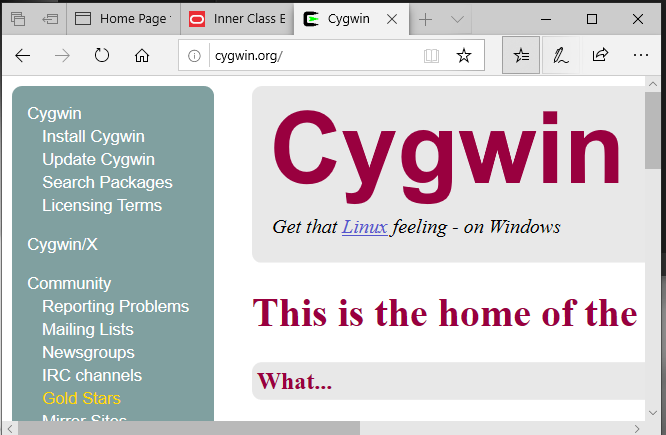
\includegraphics[width=6.0in]{../images/cygwin_00.png}
\vskip0.1in
\caption{Website for installation of Cygwin. {Screenshot} taken using
         {\bf Snip \& Sketch}. This is an app on my Windows 10 box}
\end{figure}
\eject
\vskip0.1in\hrule\vskip0.1in
\noindent
You should start with the base installation if you are not used to installing
large software packages on your computer. After the installation, there should
be an icon on your desktop that can be used to bring up a terminal emulator.
\vskip0.1in\hrule\vskip0.1in
\vfill
\begin{figure}[h]
\centering
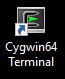
\includegraphics[width=2.0in]{../images/cygwin_icon.png}
\caption{Cygwin icon on your desktop. {Screenshot} taken using
        {\bf Snip \& Sketch}. This is an app on my Windows 10 box}
\end{figure}
\eject
\vskip0.1in\hrule\vskip0.1in
Double click on the icon and a terminal that looks like the following will
appear on your screen. The terminal comes up with a prompt that is based on the
computer name. A basic terminal will start up using the bash command terminal. 
\vskip0.1in\hrule\vskip0.1in
\vfill
\begin{figure}[h]
\centering
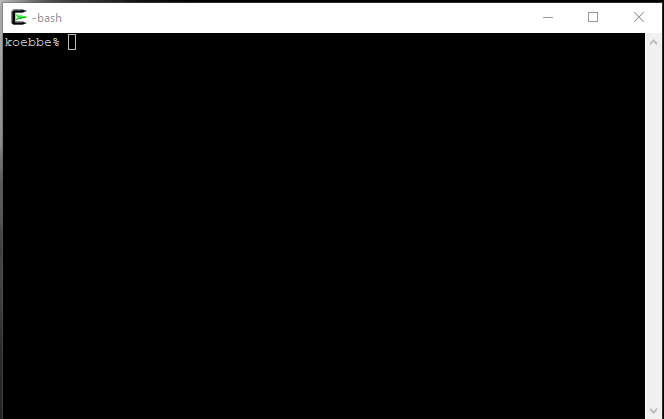
\includegraphics[width=6.0in]{../images/cygwin_01.png}
\caption{Example of a terminal that enulates a Linux operating system and
        command line. {Screenshot} taken using {\bf Snip \& Sketch}. This is
        an app on my Windows 10 box}
\end{figure}
\eject
\vskip0.1in\hrule\vskip0.1in
The text that automatically appears in the terminal is called a prompt. That
is,
\begin{verbatim}

    koebbe%

\end{verbatim}
is the prompt and our job will be to enter commands to get our computer to 
create files, modify files, compile computer programs and the like. The next
topic in our list will give you a few standard commands that can be used to
do real work for the course.
\end{document}
